
%% bare_jrnl.tex
%% V1.3
%% 2007/01/11
%% by Michael Shell
%% see http://www.michaelshell.org/
%% for current contact information.
%%
%% This is a skeleton file demonstrating the use of IEEEtran.cls
%% (requires IEEEtran.cls version 1.7 or later) with an IEEE journal paper.
%%
%% Support sites:
%% http://www.michaelshell.org/tex/ieeetran/
%% http://www.ctan.org/tex-archive/macros/latex/contrib/IEEEtran/
%% and
%% http://www.ieee.org/



% *** Authors should verify (and, if needed, correct) their LaTeX system  ***
% *** with the testflow diagnostic prior to trusting their LaTeX platform ***
% *** with production work. IEEE's font choices can trigger bugs that do  ***
% *** not appear when using other class files.                            ***
% The testflow support page is at:
% http://www.michaelshell.org/tex/testflow/


%%*************************************************************************
%% Legal Notice:
%% This code is offered as-is without any warranty either expressed or
%% implied; without even the implied warranty of MERCHANTABILITY or
%% FITNESS FOR A PARTICULAR PURPOSE! 
%% User assumes all risk.
%% In no event shall IEEE or any contributor to this code be liable for
%% any damages or losses, including, but not limited to, incidental,
%% consequential, or any other damages, resulting from the use or misuse
%% of any information contained here.
%%
%% All comments are the opinions of their respective authors and are not
%% necessarily endorsed by the IEEE.
%%
%% This work is distributed under the LaTeX Project Public License (LPPL)
%% ( http://www.latex-project.org/ ) version 1.3, and may be freely used,
%% distributed and modified. A copy of the LPPL, version 1.3, is included
%% in the base LaTeX documentation of all distributions of LaTeX released
%% 2003/12/01 or later.
%% Retain all contribution notices and credits.
%% ** Modified files should be clearly indicated as such, including  **
%% ** renaming them and changing author support contact information. **
%%
%% File list of work: IEEEtran.cls, IEEEtran_HOWTO.pdf, bare_adv.tex,
%%                    bare_conf.tex, bare_jrnl.tex, bare_jrnl_compsoc.tex
%%*************************************************************************

% Note that the a4paper option is mainly intended so that authors in
% countries using A4 can easily print to A4 and see how their papers will
% look in print - the typesetting of the document will not typically be
% affected with changes in paper size (but the bottom and side margins will).
% Use the testflow package mentioned above to verify correct handling of
% both paper sizes by the user's LaTeX system.
%
% Also note that the "draftcls" or "draftclsnofoot", not "draft", option
% should be used if it is desired that the figures are to be displayed in
% draft mode.
%
\documentclass[conference]{IEEEtran}
\usepackage{blindtext}
\usepackage{graphicx}
%\usepackage{lmodern}
\usepackage[T1]{fontenc}

% Some very useful LaTeX packages include:
% (uncomment the ones you want to load)


% *** MISC UTILITY PACKAGES ***
%
%\usepackage{ifpdf}
% Heiko Oberdiek's ifpdf.sty is very useful if you need conditional
% compilation based on whether the output is pdf or dvi.
% usage:
% \ifpdf
%   % pdf code
% \else
%   % dvi code
% \fi
% The latest version of ifpdf.sty can be obtained from:
% http://www.ctan.org/tex-archive/macros/latex/contrib/oberdiek/
% Also, note that IEEEtran.cls V1.7 and later provides a builtin
% \ifCLASSINFOpdf conditional that works the same way.
% When switching from latex to pdflatex and vice-versa, the compiler may
% have to be run twice to clear warning/error messages.






% *** CITATION PACKAGES ***
%
%\usepackage{cite}
% cite.sty was written by Donald Arseneau
% V1.6 and later of IEEEtran pre-defines the format of the cite.sty package
% \cite{} output to follow that of IEEE. Loading the cite package will
% result in citation numbers being automatically sorted and properly
% "compressed/ranged". e.g., [1], [9], [2], [7], [5], [6] without using
% cite.sty will become [1], [2], [5]--[7], [9] using cite.sty. cite.sty's
% \cite will automatically add leading space, if needed. Use cite.sty's
% noadjust option (cite.sty V3.8 and later) if you want to turn this off.
% cite.sty is already installed on most LaTeX systems. Be sure and use
% version 4.0 (2003-05-27) and later if using hyperref.sty. cite.sty does
% not currently provide for hyperlinked citations.
% The latest version can be obtained at:
% http://www.ctan.org/tex-archive/macros/latex/contrib/cite/
% The documentation is contained in the cite.sty file itself.






% *** GRAPHICS RELATED PACKAGES ***
%
\ifCLASSINFOpdf
  % \usepackage[pdftex]{graphicx}
  % declare the path(s) where your graphic files are
  % \graphicspath{{../pdf/}{../jpeg/}}
  % and their extensions so you won't have to specify these with
  % every instance of \includegraphics
  % \DeclareGraphicsExtensions{.pdf,.jpeg,.png}
\else
  % or other class option (dvipsone, dvipdf, if not using dvips). graphicx
  % will default to the driver specified in the system graphics.cfg if no
  % driver is specified.
  % \usepackage[dvips]{graphicx}
  % declare the path(s) where your graphic files are
  % \graphicspath{{../eps/}}
  % and their extensions so you won't have to specify these with
  % every instance of \includegraphics
  % \DeclareGraphicsExtensions{.eps}
\fi
% graphicx was written by David Carlisle and Sebastian Rahtz. It is
% required if you want graphics, photos, etc. graphicx.sty is already
% installed on most LaTeX systems. The latest version and documentation can
% be obtained at: 
% http://www.ctan.org/tex-archive/macros/latex/required/graphics/
% Another good source of documentation is "Using Imported Graphics in
% LaTeX2e" by Keith Reckdahl which can be found as epslatex.ps or
% epslatex.pdf at: http://www.ctan.org/tex-archive/info/
%
% latex, and pdflatex in dvi mode, support graphics in encapsulated
% postscript (.eps) format. pdflatex in pdf mode supports graphics
% in .pdf, .jpeg, .png and .mps (metapost) formats. Users should ensure
% that all non-photo figures use a vector format (.eps, .pdf, .mps) and
% not a bitmapped formats (.jpeg, .png). IEEE frowns on bitmapped formats
% which can result in "jaggedy"/blurry rendering of lines and letters as
% well as large increases in file sizes.
%
% You can find documentation about the pdfTeX application at:
% http://www.tug.org/applications/pdftex





% *** MATH PACKAGES ***
%
%\usepackage[cmex10]{amsmath}
% A popular package from the American Mathematical Society that provides
% many useful and powerful commands for dealing with mathematics. If using
% it, be sure to load this package with the cmex10 option to ensure that
% only type 1 fonts will utilized at all point sizes. Without this option,
% it is possible that some math symbols, particularly those within
% footnotes, will be rendered in bitmap form which will result in a
% document that can not be IEEE Xplore compliant!
%
% Also, note that the amsmath package sets \interdisplaylinepenalty to 10000
% thus preventing page breaks from occurring within multiline equations. Use:
%\interdisplaylinepenalty=2500
% after loading amsmath to restore such page breaks as IEEEtran.cls normally
% does. amsmath.sty is already installed on most LaTeX systems. The latest
% version and documentation can be obtained at:
% http://www.ctan.org/tex-archive/macros/latex/required/amslatex/math/





% *** SPECIALIZED LIST PACKAGES ***
%
%\usepackage{algorithmic}
% algorithmic.sty was written by Peter Williams and Rogerio Brito.
% This package provides an algorithmic environment fo describing algorithms.
% You can use the algorithmic environment in-text or within a figure
% environment to provide for a floating algorithm. Do NOT use the algorithm
% floating environment provided by algorithm.sty (by the same authors) or
% algorithm2e.sty (by Christophe Fiorio) as IEEE does not use dedicated
% algorithm float types and packages that provide these will not provide
% correct IEEE style captions. The latest version and documentation of
% algorithmic.sty can be obtained at:
% http://www.ctan.org/tex-archive/macros/latex/contrib/algorithms/
% There is also a support site at:
% http://algorithms.berlios.de/index.html
% Also of interest may be the (relatively newer and more customizable)
% algorithmicx.sty package by Szasz Janos:
% http://www.ctan.org/tex-archive/macros/latex/contrib/algorithmicx/




% *** ALIGNMENT PACKAGES ***
%
%\usepackage{array}
% Frank Mittelbach's and David Carlisle's array.sty patches and improves
% the standard LaTeX2e array and tabular environments to provide better
% appearance and additional user controls. As the default LaTeX2e table
% generation code is lacking to the point of almost being broken with
% respect to the quality of the end results, all users are strongly
% advised to use an enhanced (at the very least that provided by array.sty)
% set of table tools. array.sty is already installed on most systems. The
% latest version and documentation can be obtained at:
% http://www.ctan.org/tex-archive/macros/latex/required/tools/


%\usepackage{mdwmath}
%\usepackage{mdwtab}
% Also highly recommended is Mark Wooding's extremely powerful MDW tools,
% especially mdwmath.sty and mdwtab.sty which are used to format equations
% and tables, respectively. The MDWtools set is already installed on most
% LaTeX systems. The lastest version and documentation is available at:
% http://www.ctan.org/tex-archive/macros/latex/contrib/mdwtools/


% IEEEtran contains the IEEEeqnarray family of commands that can be used to
% generate multiline equations as well as matrices, tables, etc., of high
% quality.


%\usepackage{eqparbox}
% Also of notable interest is Scott Pakin's eqparbox package for creating
% (automatically sized) equal width boxes - aka "natural width parboxes".
% Available at:
% http://www.ctan.org/tex-archive/macros/latex/contrib/eqparbox/





% *** SUBFIGURE PACKAGES ***
%\usepackage[tight,footnotesize]{subfigure}
% subfigure.sty was written by Steven Douglas Cochran. This package makes it
% easy to put subfigures in your figures. e.g., "Figure 1a and 1b". For IEEE
% work, it is a good idea to load it with the tight package option to reduce
% the amount of white space around the subfigures. subfigure.sty is already
% installed on most LaTeX systems. The latest version and documentation can
% be obtained at:
% http://www.ctan.org/tex-archive/obsolete/macros/latex/contrib/subfigure/
% subfigure.sty has been superceeded by subfig.sty.



%\usepackage[caption=false]{caption}
%\usepackage[font=footnotesize]{subfig}
% subfig.sty, also written by Steven Douglas Cochran, is the modern
% replacement for subfigure.sty. However, subfig.sty requires and
% automatically loads Axel Sommerfeldt's caption.sty which will override
% IEEEtran.cls handling of captions and this will result in nonIEEE style
% figure/table captions. To prevent this problem, be sure and preload
% caption.sty with its "caption=false" package option. This is will preserve
% IEEEtran.cls handing of captions. Version 1.3 (2005/06/28) and later 
% (recommended due to many improvements over 1.2) of subfig.sty supports
% the caption=false option directly:
%\usepackage[caption=false,font=footnotesize]{subfig}
%
% The latest version and documentation can be obtained at:
% http://www.ctan.org/tex-archive/macros/latex/contrib/subfig/
% The latest version and documentation of caption.sty can be obtained at:
% http://www.ctan.org/tex-archive/macros/latex/contrib/caption/




% *** FLOAT PACKAGES ***
%
%\usepackage{fixltx2e}
% fixltx2e, the successor to the earlier fix2col.sty, was written by
% Frank Mittelbach and David Carlisle. This package corrects a few problems
% in the LaTeX2e kernel, the most notable of which is that in current
% LaTeX2e releases, the ordering of single and double column floats is not
% guaranteed to be preserved. Thus, an unpatched LaTeX2e can allow a
% single column figure to be placed prior to an earlier double column
% figure. The latest version and documentation can be found at:
% http://www.ctan.org/tex-archive/macros/latex/base/



%\usepackage{stfloats}
% stfloats.sty was written by Sigitas Tolusis. This package gives LaTeX2e
% the ability to do double column floats at the bottom of the page as well
% as the top. (e.g., "\begin{figure*}[!b]" is not normally possible in
% LaTeX2e). It also provides a command:
%\fnbelowfloat
% to enable the placement of footnotes below bottom floats (the standard
% LaTeX2e kernel puts them above bottom floats). This is an invasive package
% which rewrites many portions of the LaTeX2e float routines. It may not work
% with other packages that modify the LaTeX2e float routines. The latest
% version and documentation can be obtained at:
% http://www.ctan.org/tex-archive/macros/latex/contrib/sttools/
% Documentation is contained in the stfloats.sty comments as well as in the
% presfull.pdf file. Do not use the stfloats baselinefloat ability as IEEE
% does not allow \baselineskip to stretch. Authors submitting work to the
% IEEE should note that IEEE rarely uses double column equations and
% that authors should try to avoid such use. Do not be tempted to use the
% cuted.sty or midfloat.sty packages (also by Sigitas Tolusis) as IEEE does
% not format its papers in such ways.


%\ifCLASSOPTIONcaptionsoff
%  \usepackage[nomarkers]{endfloat}
% \let\MYoriglatexcaption\caption
% \renewcommand{\caption}[2][\relax]{\MYoriglatexcaption[#2]{#2}}
%\fi
% endfloat.sty was written by James Darrell McCauley and Jeff Goldberg.
% This package may be useful when used in conjunction with IEEEtran.cls'
% captionsoff option. Some IEEE journals/societies require that submissions
% have lists of figures/tables at the end of the paper and that
% figures/tables without any captions are placed on a page by themselves at
% the end of the document. If needed, the draftcls IEEEtran class option or
% \CLASSINPUTbaselinestretch interface can be used to increase the line
% spacing as well. Be sure and use the nomarkers option of endfloat to
% prevent endfloat from "marking" where the figures would have been placed
% in the text. The two hack lines of code above are a slight modification of
% that suggested by in the endfloat docs (section 8.3.1) to ensure that
% the full captions always appear in the list of figures/tables - even if
% the user used the short optional argument of \caption[]{}.
% IEEE papers do not typically make use of \caption[]'s optional argument,
% so this should not be an issue. A similar trick can be used to disable
% captions of packages such as subfig.sty that lack options to turn off
% the subcaptions:
% For subfig.sty:
% \let\MYorigsubfloat\subfloat
% \renewcommand{\subfloat}[2][\relax]{\MYorigsubfloat[]{#2}}
% For subfigure.sty:
% \let\MYorigsubfigure\subfigure
% \renewcommand{\subfigure}[2][\relax]{\MYorigsubfigure[]{#2}}
% However, the above trick will not work if both optional arguments of
% the \subfloat/subfig command are used. Furthermore, there needs to be a
% description of each subfigure *somewhere* and endfloat does not add
% subfigure captions to its list of figures. Thus, the best approach is to
% avoid the use of subfigure captions (many IEEE journals avoid them anyway)
% and instead reference/explain all the subfigures within the main caption.
% The latest version of endfloat.sty and its documentation can obtained at:
% http://www.ctan.org/tex-archive/macros/latex/contrib/endfloat/
%
% The IEEEtran \ifCLASSOPTIONcaptionsoff conditional can also be used
% later in the document, say, to conditionally put the References on a 
% page by themselves.





% *** PDF, URL AND HYPERLINK PACKAGES ***
%
%\usepackage{url}
% url.sty was written by Donald Arseneau. It provides better support for
% handling and breaking URLs. url.sty is already installed on most LaTeX
% systems. The latest version can be obtained at:
% http://www.ctan.org/tex-archive/macros/latex/contrib/misc/
% Read the url.sty source comments for usage information. Basically,
% \url{my_url_here}.





% *** Do not adjust lengths that control margins, column widths, etc. ***
% *** Do not use packages that alter fonts (such as pslatex).         ***
% There should be no need to do such things with IEEEtran.cls V1.6 and later.
% (Unless specifi


\begin{document}
%
% paper title
% can use linebreaks \\ within to get better formatting as desired
\title{Implementation of GPU based\\ Sorting Algorithms}
%
%
% author names and IEEE memberships
% note positions of commas and nonbreaking spaces ( ~ ) LaTeX will not break
% a structure at a ~ so this keeps an author's name from being broken across
% two lines.
% use \thanks{} to gain access to the first footnote area
% a separate \thanks must be used for each paragraph as LaTeX2e's \thanks
% was not built to handle multiple paragraphs
%
\author{\IEEEauthorblockN{Arvind Ramachandran}
%Reg NO: - \IEEEauthorrefmark{1}15CO111, \IEEEauthorrefmark{2}15CO112\\
\IEEEauthorblockA{Department of Computer Engineering\\
National Institute of Technology Karnataka Surathkal\\
Email: arvind0705.ar@gmail.com}
\and 
\IEEEauthorblockN{Aswanth P. P.}
\IEEEauthorblockA{Department of Computer Engineering\\
National Institute of Technology Karnataka Surathkal\\
Email: ppaswanth3@gmail.com}}

\maketitle


% note the % following the last \IEEEmembership and also \thanks - 
% these prevent an unwanted space from occurring between the last author name
% and the end of the author line. i.e., if you had this:
% 
% \author{....lastname \thanks{...} \thanks{...} }
%                     ^------------^------------^----Do not want these spaces!
%
% a space would be appended to the last name and could cause every name on that
% line to be shifted left slightly. This is one of those "LaTeX things". For
% instance, "\textbf{A} \textbf{B}" will typeset as "A B" not "AB". To get
% "AB" then you have to do: "\textbf{A}\textbf{B}"
% \thanks is no different in this regard, so shield the last } of each \thanks
% that ends a line with a % and do not let a space in before the next \thanks.
% Spaces after \IEEEmembership other than the last one are OK (and needed) as
% you are supposed to have spaces between the names. For what it is worth,
% this is a minor point as most people would not even notice if the said evil
% space somehow managed to creep in.



% The paper headers
%\markboth{Journal of \LaTeX\ Class Files,~Vol.~6, No.~1, January~2007}%
%{Shell \MakeLowercase{\textit{et al.}}: Bare Demo of IEEEtran.cls for Journals}
% The only time the second header will appear is for the odd numbered pages
% after the title page when using the twoside option.
% 
% *** Note that you probably will NOT want to include the author's ***
% *** name in the headers of peer review papers.                   ***
% You can use \ifCLASSOPTIONpeerreview for conditional compilation here if
% you desire.




% If you want to put a publisher's ID mark on the page you can do it like
% this:
%\IEEEpubid{0000--0000/00\$00.00~\copyright~2007 IEEE}
% Remember, if you use this you must call \IEEEpubidadjcol in the second
% column for its text to clear the IEEEpubid mark.



% use for special paper notices
%\IEEEspecialpapernotice{(Invited Paper)}




% make the title area
\maketitle


\begin{abstract}
Parallel sorting algorithms are widely studied nowadays. The difficulty in improving sorting run-time when run serially has lead to a lot of research in this area. Efficient sorting is required for algorithms like binary search ,merging two lists etc. The main aim is to effectively reduce the running time of these algorithms specially after the introduction of parallel processors like the GPU and CUDA, OpenCL, etc. This paper presents a survey of some well known sorting algorithms that are GPU based.
\end{abstract}
% IEEEtran.cls defaults to using nonbold math in the Abstract.
% This preserves the distinction between vectors and scalars. However,
% if the journal you are submitting to favors bold math in the abstract,
% then you can use LaTeX's standard command \boldmath at the very start
% of the abstract to achieve this. Many IEEE journals frown on math
% in the abstract anyway.

% Note that keywords are not normally used for peerreview papers.
\begin{IEEEkeywords}
Merge Sort, Quick Sort, Radix Sort, Sample Sort, Bitonic Sort, Fix Sort, GPU, CUDA
\end{IEEEkeywords}






% For peer review papers, you can put extra information on the cover
% page as needed:
% \ifCLASSOPTIONpeerreview
% \begin{center} \bfseries EDICS Category: 3-BBND \end{center}
% \fi
%
% For peerreview papers, this IEEEtran command inserts a page break and
% creates the second title. It will be ignored for other modes.
\IEEEpeerreviewmaketitle



\section{Introduction}
Sequential algorithms were implemented on a central processing unit using C++, whereas parallel algorithms were implemented on a graphics processing unit using CUDA platform. Sorting on a Central Processing Unit(CPU) is slower than sorting on a GPU.\\ 
In this Project, we analyze five parallel sorting algorithms for a given range of inputs - Merge Sort, Quick Sort, Radix Sort, Sample Sort and Bitonic Sort. Their methods are described in brief and performance compared.

\section{Objective}
We are comparing sorting time for each parallel sorting algorithm for a dataset of array size 50000 to 500000 with an interval of 5000 .The performance of each algorithm will be compared in terms of running time and corresponding graphs will be plotted for each set of inputs. 

\section{Sorting Algorithms}
We discuss a few parallel sorting algorithms here.
\subsection{Merge Sort}
Merge sort is based on the divide - and - conquer approach. It follows this approach by splitting the sequence into multiple subsequences, sorting them and then merging them into sorted sequence. If the algorithm for merging sorted sequences is stable, than the whole merge sort algorithm is also stable.

\subsection{Quick Sort}
In the Quick sort algorithm, a list of elements is taken and partitioned around a specific pivot element. The exact position of the pivot element in the sorted list is found. The lists are recursively partitioned until they become too small to partition. Quick sort is the fastest and most studied algorithm in CPU architecture.

\subsection{Radix Sort}
Radix sort is one of the fastest sorting algorithms for short keys and is the only sorting algorithm in this report which is not comparison based. Its sequential variation first splits the elements being sorted (numbers, words, dates, ...) into d r - bit digits. The elements are then sorted from least to most significant digit. For this task, the sorting algorithm has to be stable, in order to preserve the order of elements with duplicate digits.

\subsection{Sample Sort}
Sample sort is or has been the fastest sorting algorithm if the inter-process communication is high . It selects a subset of the input. This subset is referred to as splitters. Splitters are sorted by some other procedure. The input sequence is divided into buckets using these splitters. Each bucket is sorted in parallel and the result is the concatenation of these buckets. However, performance of the Sample sort degrades if the number of elements per processor is low.

\subsection{Bitonic Sort}
Bitonic Sort is one of the most studied algorithms on GPU. It falls into the group of sorting networks , which means, that the sequence and direction of comparisons is determined in advance and is independent of input sequence. Bitonic sort is based on a bitonic sequence. Parallel implementation of bitonic sort is very efficient when sorting short sequences, but it becomes slower when sorting very long sequences, because shared memory size is limited and long bionic sequences cannot be saved into it. In order to merge long bionic sequences, global memory has to be used instead of shared memory. Furthermore, global memory has to be accessed for every step of bionic merge. In order to increase the speed of sort, multiple steps of bitonic merge have to be executed with a single kernel invocation. This can be achieved with multistep bitonic sort.\\
% needed in second column of first page if using \IEEEpubid
%\IEEEpubidadjcol

% An example of a floating figure using the graphicx package.
% Note that \label must occur AFTER (or within) \caption.
% For figures, \caption should occur after the \includegraphics.
% Note that IEEEtran v1.7 and later has special internal code that
% is designed to preserve the operation of \label within \caption
% even when the captionsoff option is in effect. However, because
% of issues like this, it may be the safest practice to put all your
% \label just after \caption rather than within \caption{}.
%
% Reminder: the "draftcls" or "draftclsnofoot", not "draft", class
% option should be used if it is desired that the figures are to be
% displayed while in draft mode.
%
%\begin{figure}[!t]
%\centering
%\includegraphics[width=2.5in]{myfigure}
% where an .eps filename suffix will be assumed under latex, 
% and a .pdf suffix will be assumed for pdflatex; or what has been declared
% via \DeclareGraphicsExtensions.
%\caption{Simulation Results}
%\label{fig_sim}
%\end{figure}

% Note that IEEE typically puts floats only at the top, even when this
% results in a large percentage of a column being occupied by floats.


% An example of a double column floating figure using two subfigures.
% (The subfig.sty package must be loaded for this to work.)
% The subfigure \label commands are set within each subfloat command, the
% \label for the overall figure must come after \caption.
% \hfil must be used as a separator to get equal spacing.
% The subfigure.sty package works much the same way, except \subfigure is
% used instead of \subfloat.
%
%\begin{figure*}[!t]
%\centerline{\subfloat[Case I]\includegraphics[width=2.5in]{subfigcase1}%
%\label{fig_first_case}}
%\hfil
%\subfloat[Case II]{\includegraphics[width=2.5in]{subfigcase2}%
%\label{fig_second_case}}}
%\caption{Simulation results}
%\label{fig_sim}
%\end{figure*}
%
% Note that often IEEE papers with subfigures do not employ subfigure
% captions (using the optional argument to \subfloat), but instead will
% reference/describe all of them (a), (b), etc., within the main caption.


% An example of a floating table. Note that, for IEEE style tables, the 
% \caption command should come BEFORE the table. Table text will default to
% \footnotesize as IEEE normally uses this smaller font for tables.
% The \label must come after \caption as always.
%
%\begin{table}[!t]
%% increase table row spacing, adjust to taste
%\renewcommand{\arraystretch}{1.3}
% if using array.sty, it might be a good idea to tweak the value of
% \extrarowheight as needed to properly center the text within the cells
%\caption{An Example of a Table}
%\label{table_example}
%\centering
%% Some packages, such as MDW tools, offer better commands for making tables
%% than the plain LaTeX2e tabular which is used here.
%\begin{tabular}{|c||c|}
%\hline
%One & Two\\
%\hline
%Three & Four\\
%\hline
%\end{tabular}
%\end{table}


% Note that IEEE does not put floats in the very first column - or typically
% anywhere on the first page for that matter. Also, in-text middle ("here")
% positioning is not used. Most IEEE journals use top floats exclusively.
% Note that, LaTeX2e, unlike IEEE journals, places footnotes above bottom
% floats. This can be corrected via the \fnbelowfloat command of the
% stfloats package.

\section{Project Timeline }
This is the proposed timeline which we hope to achieve : 
27th September 2017 - Discussion of Project Proposal\\
2nd October 2017 - Submission of Proposal\\
23rd October 2017 - Mid Progress Evaluation\\
13th November 2017 - Final Demo\\
24th November 2017 - Report Submission\\

\section{Work Distribution}
This is how we plan to split the work and proceed with the Project.
The work has been divided equally among the team.
\subsection{Arvind Ramachandran (15CO111)}
Implementation and Analysis of Merge Sort and Sample Sort.
\subsection{Aswanth P P (15CO112)}
Implementation and Analysis of Quick Sort and Radix Sort.\\
Bitonic Sort has been done by both of us together. 

\section{GPU Sorting Algorithms}
Merge sort, Radix sort, Quick sort, Sample sort and Bitonic sort algorithms were successfully implemented on CUDA , running times calculated and results verified using functions from header "wb.h".

\subsection{Merge Sort}
Conceptually, a merge sort works as follows:   \\1) Divide the unsorted list into n sublists, each containing 1 element (a list of 1 element is considered sorted).\\
   2) Repeatedly merge sublists to produce new sorted sublists until there is only 1 sublist remaining. This will be the sorted list.\\
   
   Since this follows a divide and conquer approach, each sort and merge operation is performed individually (recursively as per the algorithm)
 which takes up time. There arises a need to parallelize this algorithm in order to improve its efficiency. Merge sort parallelizes well due to use of the divide-and-conquer method. It is very difficult to find a merging algorithm that can achieve
a high level of parallelism and maximize utilization on the GPU due to the multi-level parallelism requirements of the
architecture. In a sense, parallelizing merging algorithms is
even more difficult due to the small amount of work done
per each element in the input and output. The merge phase
of the original Merge Path algorithm is not well-suited for
the GPU as the merging stage is purely sequential for each
core. Therefore, it is necessary to extend the algorithm to
parallelize the merge stage in a way that still uses all the
SPs on each SM once the partitioning stage is completed. For full utilization of the SMs in the system, the merge
must be broken up into finer granularity to enable additional
parallelism while still avoiding synchronization when possible. \\

\begin{figure}[h]
\[\includegraphics[scale=0.55]{merge.png}\]
\caption{An example of the execution of merge sort.}
\end{figure}

We have adopted the following strategy to parallelize merge sort :\\
1) Start with two lists: Your input array, and a temp array that’s the same size.\\
2) Define a width, starting at 2. During each step, width gets multiplied by 2.\\
3) While width is less than 2N, sort each width-sized chunk of the list into the temp list. Then switch the pointers of the two lists. We thereby avoid allocating small arrays or copying temp back to input.\\

NOTE : This is the step that happens in parallel. Each thread gets a
chunk of the list to sort.
Two halves of each chunk are are sorted / merged against
each other into the temp array.\\

4) We end up with one big chunk being sorted into the final list, and you switch input and temp one last time, returning temp.

\subsection{Radix Sort}
Radix Sort iterates over the keys bits from the least-
significant to the most-significant digit, considering an
implementation specific number of consecutive bits at a time.
With each sorting pass, a stable counting sort is used to partition the keys into buckets according to the bits being
considered with the current pass. The stable counting sort
computes each keys offset by counting the number of keys
with a smaller digit value and, as it needs to be stable,
the keys with the same digit value preceding the key in
the input sequence.
Sorting relies on the reinterpretation of a
k-bit key
as a sequence of
d-bit digits, which are considered one at
a time. The basic idea is, that splitting the
k
bits of the
keys into smaller
d-bit digits results in a small enough radix
r
= 2
d
, such that the keys can efficiently be partitioned
into
r
distinct buckets. As sorting on each digit can be
done with an effort that is linear in the number of keys
n
,
the whole sorting can be achieved with a total complexity of
O
(
dk/de*n
). Iterating over the keys’ digits can be
performed in two fundamentally different ways. Either by
proceeding from the most-significant to the least-significant
digit (MSD radix sort), or vice versa (LSD radix sort). Radix sort is an out-of-place sort and we need to ping-pong
values between the input and output buffers provided. We
need to do a copy at the end.\\

The basic idea is to construct a histogram on each pass
of how many of each ”digit” there are. Then we scan this
histogram so that we know where to put the output of each
digit. For example, the first 1 must come after all the 0s so
we have to know how many 0s there are to be able to start
moving 1s into the correct position.
\\1) Histogram of the number of occurrences of each digit
\\2) Exclusive Prefix Sum of Histogram
\\3) Determine relative offset of each digit
For example [0 0 1 1 0 0 1] = [0 1 0 1 2 3 2]
\\4) Combine the results of steps 2 3 to determine the final
output location for each element and move it there LSB.
\begin{figure}[h]
\[\includegraphics[scale=0.38]{radix.jpg}\]
\caption{Parallel Radix Sort on the GPU}
\end{figure}

Implementation of Radix on CUDA algorithm:
\\1) Get the predicate of your list (bit in common, starting
from the LSB)
\\2) Scan the predicate, and record the sum of the predicate in
the process
Implement Scan on the GPU
Note that your predicate will be of arbitrary size
\\3) Flip bits of the predicate, and scan that
\\4) Move the values in your array with the following rule:
For the i\textsuperscript{th} element in the array:
if the i\textsuperscript{th} predicate is TRUE, move the i\textsuperscript{th} value to the index
in the i\textsuperscript{th} element of the predicate scan
else, move the i\textsuperscript{th} value to the index in the i\textsuperscript{th} element of the
!Predicate scan plus the sum of the Predicate
\\5) Move to the next significant bit (NSB)\\

Verification of the radix sort algorithm is done by using "wb.h" library where the result was compared with existing sorted elements file.which gave the following result for the execution of 50000 elements within range of 5000.
A sample of the working is as follows :\\


 Generic 0.030998016 Importing data to host\\

 GPU     0.000162048 Allocating GPU memory.\\

 GPU     0.000172800 Copying input memory to the GPU.\\

 Compute 0.039742976 Performing CUDA computation\\

 Copy    0.000344832 Copying output memory to the CPU\\

 GPU    0.000151040 Freeing GPU Memory\\

 Solution is correct.\\

\subsection{Quick Sort}
In the Quick sort algorithm, a list of elements is taken and partitioned around a specific pivot element. The exact position of the pivot element in the sorted list is found. The lists are recursively partitioned until they become too small to partition. Quick sort is the fastest and most studied algorithm in CPU architecture.\\

The algorithm is suitable for segmented
scan primitive due to communications between elements (threads) inside a
single segment. A pivot element is chosen in each segment (the first element of the
segment). The pivot element is distributed across the segments. The input element is
compared to the pivot.Greater-than or greater-than-or-equal are compared accordingly
in alternating passes of the algorithm. A segmented vector containing true and false
is produced by the comparison operation. This segmented vector is used to split and segment the input. As a result, smaller elements are placed at the head of the vector
and larger elements are placed at the end of the vector. \\

A sequence to be partitioned is divided logically into sections. Each section is
processed by a thread block. Each thread in the thread block keeps track of the number
of elements it has seen larger and smaller than the pivot. Each thread stores this
information in two arrays in shared local memory. A cumulative sum is calculated to
find out the index of each element. Threads will write their assigned elements in new
position in the auxiliary buffer.When the number of sub-sequences is large enough that
each thread block can be assigned one, the algorithm enters in the second phase. There
is no need for inter-thread block synchronization. When the sub-sequences become
small enough to be sorted entirely in the fast local memory, the authors suggest using
a different sorting algorithm which performs well when the size of the list approaches
the number of threads.\\

One kernel is assigned to the group having elements smaller than the pivot
and the other is assigned to the group having elements larger than the pivot. The kernel
at the top knows the index and the size of the two groups; it will have the information
on whether to launch a kernel and how many threads to use. The parent kernel is able to
launch its child kernels immediately after partitioning the list. The program progresses
in an asynchronous manner. The kernel launches its two children in a separate stream.
CUDA streams are executed simultaneously, which means the two sub-sorts will run
in parallel.\\

Input Size : 50000 

Execution Time : 0. 51

Input Size/Execution Time : 98039\\

\subsection{Sample Sort}
Sample sort is or has been the fastest sorting algorithm if the inter-process communication is high. It selects a subset of the input. This subset is referred to as splitters. Splitters are sorted by some other procedure. The input sequence is divided into buckets using these splitters. Each bucket is sorted in parallel and the result is the concatenation of these buckets. However, performance of the Sample sort degrades if the number of elements per processor is low.\\

The idea behind sample sort is simple. A sample of size s is selected from the n-element sequence, and the range of the buckets is determined by sorting the sample and choosing m - 1 elements from the result. These elements (called splitters) divide the sample into m equal-sized buckets. After defining the buckets, the algorithm proceeds in the same way as bucket sort. The performance of sample sort depends on the sample size s and the way it is selected from the n-element sequence.\\

Consider a splitter selection scheme that guarantees that the number of elements ending up in each bucket is roughly the same for all buckets. Let n be the number of elements to be sorted and m be the number of buckets. The scheme works as follows. It divides the n elements into m blocks of size n/m each, and sorts each block by using quicksort. From each sorted block it chooses m - 1 evenly spaced elements. The m(m - 1) elements selected from all the blocks represent the sample used to determine the buckets. This scheme guarantees that the number of elements ending up in each bucket is less than 2n/m.\\

How can we parallelize the splitter selection scheme? Let p be the number of processes. As in bucket sort, set m = p; thus, at the end of the algorithm, each process contains only the elements belonging to a single bucket. Each process is assigned a block of n/p elements, which it sorts sequentially. It then chooses p - 1 evenly spaced elements from the sorted block. Each process sends its p - 1 sample elements to one process - say P0. Process P0 then sequentially sorts the p(p - 1) sample elements and selects the p - 1 splitters. Finally, process P0 broadcasts the p - 1 splitters to all the other processes.\\

Since the algorithm spends a significant
amount of time on sorting buckets (for example approximately
55 percentage for sorting 16 million randomly distributed
32-bit integers) one should not underestimate influence of
this step on the overall run-time of the algorithm. We delay
sorting of buckets until the whole input is partitioned into
buckets of size at most M. Since the number of buckets
grows with the input size, it is larger than the number of
processors in most of the cases. Therefore, we can use a
single thread block per bucket without sacrificing exploitable
parallelism. To improve load-balancing we schedule buckets
for sorting ordered by size.\\

In order to sort buckets efficiently we split them into
chunks that fit into shared memory, which then can be
sorted without expensive accesses to the global memory.
Initially we employed a sample sort based algorithm for
this purpose. But we found that it performed slightly worse
than our quick sort adaptation by Cederman and Tsigas,
which we therefore use in our final implementation. We
also extended it to support key-value pairs inputs. Quick sort
does not cause any serialization of work, except for pivot
selection and stack operations. Additionally, its consumption
of registers and shared memory is modest. \\


\begin{figure}[h]
\[\includegraphics[scale=0.45]{sample.png}\]
\caption{An example of the execution of sample sort on an array with 24 elements on three processes.}
\end{figure}
 By choosing t = 256 threads per block and = 8
elements per thread, we achieve a compromise between the
parallelism exposed by the algorithm, the amount of data
(n·k)/(t·) written in the second phase and memory latency
in the fourth phase.\\

Input Size : 50000

Execution Time : 0. 09

Input Size/Execution Time : 555555

\subsection{Bitonic Sort}
The bitonic sorting scheme has been extensively used in
parallel computing (mainly to construct sorting network).
Bitonic sort with the property that sequence of comparisons is
data-independent. Therefore it is one of the fastest parallel
sorting algorithms. There are two steps in bitonic sorting
algorithm. Firstly, it makes the arbitrary sequence that is
called bitonic sequence. Secondly, it can be converted to the
first one by cyclically shifting. Bitonic sequence consists
of two monotonic sequences. The monotonic sequence is
increase or decrease from left to right.\\

For all k < n; If a\textsubscript{k} < a\textsubscript{k+1} ; a\textsubscript{1}, a\textsubscript{2}, a\textsubscript{3}...a\textsubscript{n} is a monotonic
sequence. Bitonic sequence monotonically increases
(decreases), reaches the maximum (minimum), then
monotonically decreases (increases). For example, suppose 3
5 8 9 7 4 2 1 bitonic sequence; it increases from 3 to 9 then it
decreases. If x\textsubscript{0}, x\textsubscript{1}, x\textsubscript{2}...x\textsubscript{n} is a bitonic sequence, an index i is
between 0<i<n-1. When we apply this rule to sequence, it
increases from x\textsubscript{0} to x\textsubscript{i} , then decreases from x\textsubscript{i} to x\textsubscript{n} . Bitonic
split is applied to sequence to get a bitonic sequence. The
sequence length must be 2n. Then, n steps are needed to sort
the entire array. Each indices are compared using (i, n/2-1). If
a\textsubscript{i} > a\textsubscript{i+n/2}, the two elements are exchanged, 1<i<n . When
this swapping operation is applied to indices between i=(0,
n/2-1), two bitonic sequences are produced. The first split
elements are smaller than second split elements. Then, in the second step the same rule will be applied to
each subsequence. Each subsequence will produce new
subsequence. When n step is applied, it produces the
subsequence of length 1. Finally, all the elements in the
bitonic sequence will be sorted.\\

\begin{figure}[h]
\includegraphics[scale=0.5]{bitonic_build_2.png}
\caption{Bitonic Sorting Network}
\end{figure}
Bitonic sort consists of O(n(logn)) 2 comparison operation
(compare/exchange) in each n/2 step. Total number of steps
are k=log(n). When this algorithm is parallelized, it would
take n processor to sort it with O(logn) 2 complexity. All steps
in bitonic sort are creating a bitonic sequence and the sorting
are (k(k+1))/2. For example the sorting of an array that consist
16 elements (2 4 ) would take 10 steps. Firstly, pair wise exchange is made to
make it easier to find the bitonic sequence. Then, it is divided
two sub-arrays. Each element in sub-array is compared using
(i,n/2-1) indices. If a\textsubscript{i} > a\textsubscript{i+n/2} , swap operation is applied. After
all elements are compared, bitonic sequence is implemented.
The first split of the array is in increasing order; the second
split is in decreasing order. It is reached to bitonic sequence in
3 steps. Next step is the bitonic sorting. These 2 bitonic splits
are divided again until each split that will have 1 element.
Compare and swap approach is applied to all splits. Finally,
bitonic sorted array is implemented.\\

In parallel implementation of this sorting algorithm, each
split and compare operation is applied on different cores. Each
core works on different part of an array. These splitted arrays
results don't affect the other one's result. Therefore, each
CUDA core works on array separately.

\section{Performance Analysis}
We have compared the running times of these sorting algorithms over an input size ranging from 10000 to 50000. We have plotted a graph of Running time against Input Size as follows:
\begin{figure}[h]
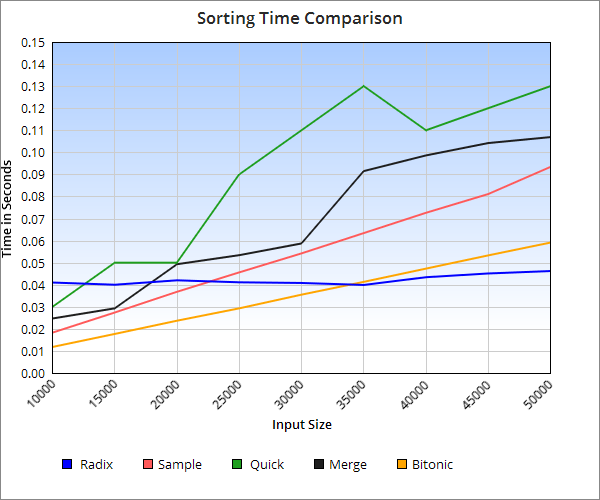
\includegraphics[scale=0.4]{NewLineGraph.png}
\caption{Sorting Time Comparison}
\end{figure}
\section{Conclusion}
This paper presented a survey of GPU based sorting algorithms. We have selected five sorting algorithms for this purpose - Merge sort, Radix sort, Sample sort, Quick sort and Bitonic sort. Working and performances of these algorithms have been calculated and compared. Our analysis showed that all these performed better than their serial counterparts. Due to the highly
optimal complexity of Radix sort, it is a difficult to outrival algorithm on GPU. In the future, we will try to extend our algorithms
and try other sorting algorithms to compare these algorithms’s
performance. Different data ranges and distribution can be
applied to these algorithms in both academic and industrial
fields based on the use of GPU. Finally, we will compare the results for
more GPU compute capabilities and propose an algorithm to
automatically choose the best one for each input parameters.

\begin{thebibliography}{1}

\bibitem{IEEEhowto:niels}
Sam~White, Niels~Verosky and Tia~Newhall, "A CUDA-MPI Hybrid Bitonic Sorting Algorithm for GPU Clusters", in \emph{41st International Conference on Parallel Processing Workshops}, 2012.
\\
\bibitem{IEEEhowto:zehra}
Zehra~Yildiz, Musa~Aydin and Guray~Yilmaz, "Parallelization of bitonic sort and radix sort algorithms on many core GPUs".
\\
\bibitem{IEEEhowto:bakulev}
Bakulev~Aleksander~Valerievich, Bakuleva~Marina~Alekseevna, Pyurova~Tatiana~Anatolievna and Skvortsov~Sergei~Vladimirovich, "The Implementation on CUDA Platform Parallel
Algorithms Sort the Data", in \emph{6th Mediterranean Conference on Embedded Computing}, 2017.
\\
\bibitem{IEEEhowto:nikolaj}
Nikolaj~Leischner, Vitaly~Osipov and Peter~Sanders, "GPU Sample Sort", in \emph{Parallel \& Distributed Processing (IPDPS), IEEE
International Symposium}, 2010.
\\
\bibitem{IEEEhowto:rafael}
Rafael~Schmid, Edson~Borin, Edson~Caceres and Flavia~Pisani, "An Evaluation of Segmented Sorting Strategies on GPUs", in \emph{14th IEEE International Conference on Smart City}; \emph{IEEE 2nd International Conference on Data Science and Systems}; \emph{18th IEEE International Conference on High Performance Computing anf Communications}, 2016.
\\
\bibitem{IEEEhowto:dhirendra}
Dhirendra~Pratap~Singh, Ishan~Joshi and Jaytrilok~Choudhary, "Survey of GPU Based Sorting Algorithms", 2017.
\\
\bibitem{IEEEhowto:pdf}
http://docs.nvidia.com/cuda/pdf/CUDA\_C\_Programming\_Guide.pdf

\end{thebibliography}

\end{document}



